%----------------------------------------------------------------------------------------
%	PACKAGES AND OTHER DOCUMENT CONFIGURATIONS
%----------------------------------------------------------------------------------------
\documentclass{article}
\usepackage{mathtools}
\usepackage{tikz}
\usetikzlibrary{backgrounds}
%\usepackage{kbordermatrix}
\usepackage{float}
\usepackage{amsmath,amsfonts,amsthm} % Math packages
\setlength\parindent{0pt} % Removes all indentation from paragraphs - comment this line for an assignment with lots of text

%----------------------------------------------------------------------------------------
%	TITLE SECTION
%----------------------------------------------------------------------------------------

\newcommand{\horrule}[1]{\rule{\linewidth}{#1}} % Create horizontal rule command with 1 argument of height

\title{	
\normalfont \normalsize
\textsc{North Carolina State University, CSC565 Spring 2018} \\
\horrule{0.5pt} \\[0.4cm] % Thin top horizontal rule
\huge Homework \#2 \\ % The assignment title
\horrule{2pt} \\[0.5cm] % Thick bottom horizontal rule
}
\author{Team H: asfadnav, lle3, lzhou15, ssaffar} % Your name
\date{\normalsize\today} % Today's date or a custom date
\begin{document}

\maketitle % Print the title

%----------------------------------------------------------------------------------------
%	PROBLEM 1
%----------------------------------------------------------------------------------------
\section*{Problem 1}

Linfeng
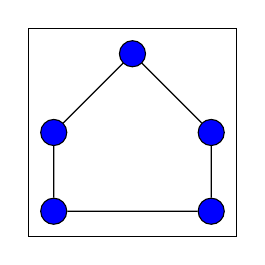
\begin{tikzpicture}[framed, every node/.style={draw,shape=circle,fill=blue,text=white}]
		\path (0,0) node (p0) {}
		(-1,-1) node (p4) {}
		(1, -1) node (p1) {}
		(-1, -2) node (p3) {}
		(1, -2) node (p2) {};

		\draw (p0) -- (p1)
		(p1) -- (p2)
		(p2) -- (p3)
		(p3) -- (p4)
		(p4) -- (p0);

	\end{tikzpicture}
%----------------------------------------------------------------------------------------
%	PROBLEM 2
%----------------------------------------------------------------------------------------
\section*{Problem 2}

	The following 6 graphs show all the isomorphism classes of simple graphs with 5 vertices and 5 edges. \\

	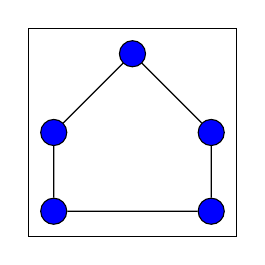
\begin{tikzpicture}[framed, every node/.style={draw,shape=circle,fill=blue,text=white}]
		\path (0,0) node (p0) {}
		(-1,-1) node (p4) {}
		(1, -1) node (p1) {}
		(-1, -2) node (p3) {}
		(1, -2) node (p2) {};

		\draw (p0) -- (p1)
		(p1) -- (p2)
		(p2) -- (p3)
		(p3) -- (p4)
		(p4) -- (p0);

	\end{tikzpicture}
	\hspace{.25cm}
	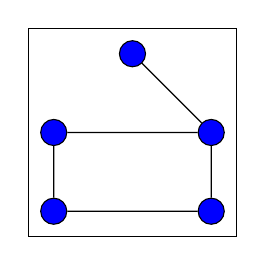
\begin{tikzpicture}[framed, every node/.style={draw,shape=circle,fill=blue,text=white}]
		\path (0,0) node (p0) {}
		(-1,-1) node (p4) {}
		(1, -1) node (p1) {}
		(-1, -2) node (p3) {}
		(1, -2) node (p2) {};

		\draw (p0) -- (p1)
		(p1) -- (p2)
		(p2) -- (p3)
		(p3) -- (p4)
		(p4) -- (p1);

	\end{tikzpicture}
	\hspace{.25cm}
	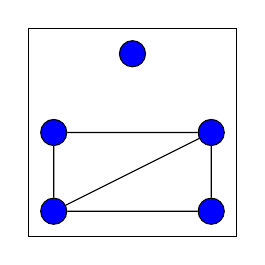
\begin{tikzpicture}[framed, every node/.style={draw,shape=circle,fill=blue,text=white}]
		\path (0,0) node (p0) {}
		(-1,-1) node (p4) {}
		(1, -1) node (p1) {}
		(-1, -2) node (p3) {}
		(1, -2) node (p2) {};

		\draw (p1) -- (p3)
		(p1) -- (p2)
		(p2) -- (p3)
		(p3) -- (p4)
		(p4) -- (p1);
	\end{tikzpicture}

	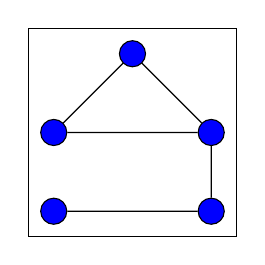
\begin{tikzpicture}[framed, every node/.style={draw,shape=circle,fill=blue,text=white}]
		\path (0,0) node (p0) {}
		(-1,-1) node (p4) {}
		(1, -1) node (p1) {}
		(-1, -2) node (p3) {}
		(1, -2) node (p2) {};

		\draw (p0) -- (p1)
		(p1) -- (p2)
		(p2) -- (p3)
		(p1) -- (p4)
		(p4) -- (p0);
	\end{tikzpicture}
	\hspace{.25cm}
	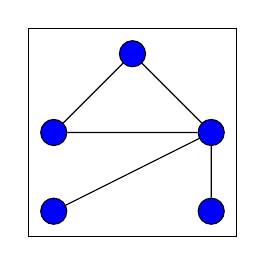
\begin{tikzpicture}[framed, every node/.style={draw,shape=circle,fill=blue,text=white}]
		\path (0,0) node (p0) {}
		(-1,-1) node (p4) {}
		(1, -1) node (p1) {}
		(-1, -2) node (p3) {}
		(1, -2) node (p2) {};

		\draw (p0) -- (p1)
		(p1) -- (p2)
		(p1) -- (p3)
		(p1) -- (p4)
		(p4) -- (p0);
	\end{tikzpicture}
	\hspace{.25cm}
	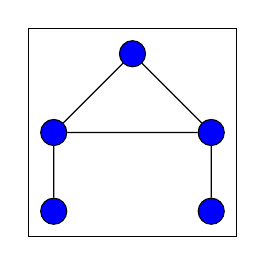
\begin{tikzpicture}[framed, every node/.style={draw,shape=circle,fill=blue,text=white}]
		\path (0,0) node (p0) {}
		(-1,-1) node (p4) {}
		(1, -1) node (p1) {}
		(-1, -2) node (p3) {}
		(1, -2) node (p2) {};

		\draw (p0) -- (p1)
		(p1) -- (p2)
		(p4) -- (p3)
		(p1) -- (p4)
		(p4) -- (p0);
	\end{tikzpicture}

%----------------------------------------------------------------------------------------
%	PROBLEM 3
%----------------------------------------------------------------------------------------
\section*{Problem 3}
		
The first two graphs are isomorphic and bipartite, and have no odd cycle. The third graph is not bipartite and has an odd cycle, and so it is not isomorphic to the others. We can show the first two graphs are isomorphic by relabeling the vertices of the second graph.

The first graph is as below.

\begin{figure}[H]
\centering
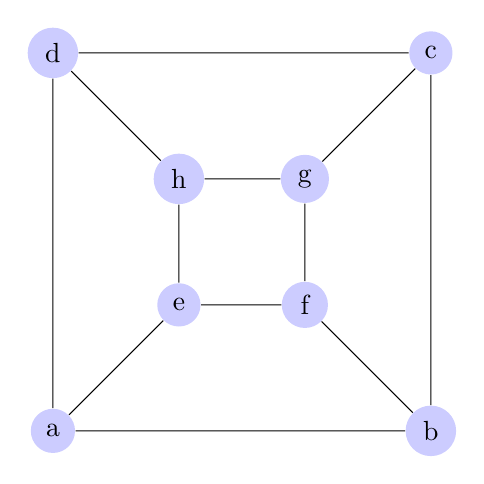
\begin{tikzpicture}
  [scale=.8,auto=center,every node/.style={circle,fill=blue!20}]
  \node (a) at (2,2) {a};
  \node (b) at (8,2)  {b};
  \node (c) at (8,8)  {c};
  \node (d) at (2,8) {d};
  \node (e) at (4,4)  {e};
  \node (f) at (6,4)  {f};
  \node (g) at (6,6) {g};
  \node (h) at (4,6) {h};

  \foreach \from/\to in {a/b,b/c,c/d,d/a,a/e,b/f,c/g,d/h,e/f,f/g,g/h,h/e}
    \draw (\from) -- (\to);
\end{tikzpicture}
\caption{Graph $G_1$}
\end{figure}

After relabeling the vertices of the second graph, it becomes as the graph below which is same as the first graph. Hence, the first and the second graph are isomorphic.

\begin{figure}[H]
\centering
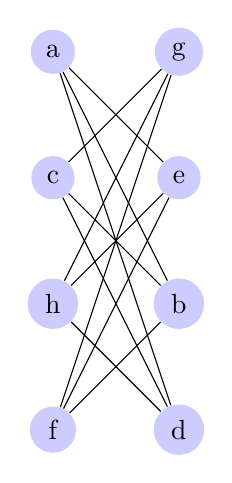
\begin{tikzpicture}
  [scale=.8,auto=center,every node/.style={circle,fill=blue!20}]
  \node (a) at (2,8) {a};
  \node (b) at (4,4)  {b};
  \node (c) at (2,6)  {c};
  \node (d) at (4,2) {d};
  \node (e) at (4,6)  {e};
  \node (f) at (2,2)  {f};
  \node (g) at (4,8) {g};
  \node (h) at (2,4) {h};

  \foreach \from/\to in {a/b,b/c,c/d,d/a,a/e,b/f,c/g,d/h,e/f,f/g,g/h,h/e}
    \draw (\from) -- (\to);
\end{tikzpicture}
\caption{Graph $G_2$}
\end{figure}

%----------------------------------------------------------------------------------------
%	PROBLEM 4
%----------------------------------------------------------------------------------------
\section*{Problem 4}
		
Since $A$ is the adjacency matrix of $K_n$, the diagonal elements of $A$ are all zero, and all non-diagonal elements of $A$ are 1, as below.

\[A_{n\times n}=\begin{bmatrix}
  0&1&1&\hdots&1 \\
  1&0&1&\hdots&1\\
   \vdots& \ddots & \ddots & \ddots &\vdots\\
  1&\hdots&1&0&1\\
  1&\hdots&1&1&0
  \end{bmatrix}\]

  Let the matrix $B$ be a $n\times n$ matrix with all elements 1, as below.

  \[B_{n\times n}=\begin{bmatrix}
 1&1&\hdots&1 \\
  1&\ddots&\ddots&\vdots\\
   \vdots& \ddots & \ddots & 1\\
  1&\hdots&1&1
  \end{bmatrix}\]

  We can write $A$ as $A=B-I_n$. Now, we have

  $$A^2=(B-I_n)^2=(B-I_n)\times (B-I_n)=B^2-2B+I_n^2=B^2-2B+I_n$$

  With matrix $B$ defined as above, we have the $B^2$ as a $n\times n$ matrix with all elements equal to $n$, as below.

    \[
B^2=\begin{bmatrix}
 n&n&\hdots&n \\
  n&\ddots&\ddots&\vdots\\
   \vdots& \ddots & \ddots &n\\
  n&\hdots&n&n
  \end{bmatrix}
  \]

  Therefore,

   \[
A^2=B^2-2B+I_n=\begin{bmatrix}
 n&n&\hdots&n \\
  n&\ddots&\ddots&\vdots\\
   \vdots& \ddots & \ddots &n\\
  n&\hdots&n&n
  \end{bmatrix}
  -
  \begin{bmatrix}
 2&2&\hdots&2 \\
  2&\ddots&\ddots&\vdots\\
   \vdots& \ddots & \ddots &2\\
  2&\hdots&2&2
  \end{bmatrix}
  +
  \begin{bmatrix}
 1&0&\hdots&0 \\
  0&\ddots&\ddots&\vdots\\
   \vdots& \ddots & \ddots &0\\
  0&\hdots&0&1
  \end{bmatrix}
  \]

  \[A^2=\begin{bmatrix}
  n-1&n-2&n-2&\hdots&n-2 \\
  n-2&n-1&n-2&\hdots&n-2\\
   \vdots& \ddots & \ddots & \ddots &\vdots\\
  n-2&\hdots&n-2&n-1&n-2\\
  n-2&\hdots&n-2&n-2&n-1
  \end{bmatrix}\]

  Hence,

  \begin{equation*}
  A^2[i,j] =
    \begin{cases}
      n-1 & \text{if $i=j$}\\
      n-2 & \text{if $i\neq j$}
    \end{cases}
\end{equation*}

%----------------------------------------------------------------------------------------
%	PROBLEM 5
%----------------------------------------------------------------------------------------
\section*{Problem 5}
		
This statement is true. If $G$ is a disconnected graph, then $\overline{G}$, the complement is connected. \\

To prove this, let's say we have two vertices,  $u$ and $v$,  in graph $G$. \\

In one scenario $u$ and $v$ are parts of different connected sub-graphs. This means in graph $G$, there is no $\{u,v\}$ edge, but in $\overline{G}$ there will be one. \\

Now let's assume a different scenario where u and v are in the same connected sub-graph in $G$. Then there must exist a vertex $w$ such that it is in a different connected sub-graph since $G$ is disconnected.
So in $\overline{G}$, there will be an edge $\{u,w\}$ and $\{v,w\}$. Even though in $\overline{G}$, $\{u,v\}$ will no longer exist, there will be a path going $\{u,w\}$, $\{w,v\}$ so u and v are still connected. \\

With this logic, any two vertices will be connectedin $\overline{G}$, so the whole graph will be connected.

%----------------------------------------------------------------------------------------
%	PROBLEM 6
%----------------------------------------------------------------------------------------
\section*{Problem 6}

Linfeng

\begin{figure}[H]
\centering
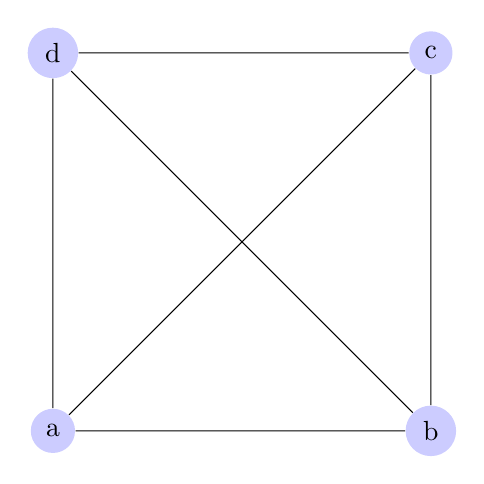
\begin{tikzpicture}
  [scale=.8,auto=center,every node/.style={circle,fill=blue!20}]
  \node (a) at (2,2) {a};
  \node (b) at (8,2)  {b};
  \node (c) at (8,8)  {c};
  \node (d) at (2,8) {d};

  \foreach \from/\to in {a/b,b/c,c/d,d/a,a/c,b/d}
    \draw (\from) -- (\to);
\end{tikzpicture}
\caption{Graph $K_4$}
\end{figure}
\begin{itemize}
\item \(K_4\) has a walk that is not a trail. For example, \((a,b,a)\) is a walk but is not a trail. 
\item \(K_4\) has a trail that is not closed and is not a path. Path contains no repeated vertex and trail has no repeated edge. We can find \((c,a,d,c,b)\) is a trail that is not closed and is not a path.
\item Every single vertex is a closed trail that is not a cycle. A closed trail has even vertex degrees, so for \(K_4\) we require degree 2 or 0, for those vertices with degree 2, it's impossible to find a closed trail that is not a cycle every such trail is a cycle in a complete graph. Therefore, in conclusion, a single vertex forms a closed trail that is not a cycle. 


\end{itemize}


%----------------------------------------------------------------------------------------
%	PROBLEM 7
%----------------------------------------------------------------------------------------
\section*{Problem 7}


		A graph is called \textit{chordal} if it has no induced subgraph isomorphic to $C_n$ for any $n>=4$.
		\begin{enumerate}
			\item $K_{10}$: Chordal\\
			because,\\
			Every induced subgraph of $K_{10}$ can only be $K_n$, $4 <= n <= 10$ and therefore can never be a cycle.\\
			
			\item $K_{5,5}$: Not chordal\\
			because,\\
			This graph has a subgraph $K_{2,2}$, which is isomorphic to $C_4$.\\

			\item $K_{1,9}$: Chordal\\
			because,\\
			This is basically a claw, and can therefore have no subgraph isomorphic to any cycle.\\
			
			\item $C_{10}$: Not chordal\\
			because,\\
			This graph is its own induced subgraph that is isomorphic to $C_{10}$.\\

			\item $P_{10}$: Chordal\\
			because,\\
			A path cannot have a repeated vertex and can therefore not have a cycle. By extension, none of its subgraphs can have a cycle.\\

			\item the Petersen graph: Not chordal\\
			because,\\
			Its outer pentagon is an induced subgraph that is $C_5$.\\
		\end{enumerate}
		
%----------------------------------------------------------------------------------------
%	PROBLEM 8
%----------------------------------------------------------------------------------------
%\section*{Problem 8}
%		\begin{enumerate}
%			\item Incidence matrices for the given graphs:
%			\begin{enumerate}
%				\item Graph 1
%				\kbordermatrix
%				{
%    					& e_1	& e_2	\\
%    				v_1	& 1		& 0		\\
%    				v_2	& 1		& 1		\\
%    				v_3	& 0		& 1		\\
%    				v_4	& 0		& 0		\\
%    			}
%    			
%    			\item Graph 2
%				\kbordermatrix
%				{
%    					& e_1	& e_2	& e_3	& e_4	\\
%    				v_1	& 1		& 0		& 1		& 0		\\
%    				v_2	& 1		& 1		& 0		& 0		\\
%    				v_3	& 0		& 1		& 1		& 1		\\
%    				v_4	& 0		& 0		& 0		& 1		\\
%    			}
%    			
%    			\item Graph 3
%				\kbordermatrix
%				{
%    					& e_1	& e_2	& e_3	& e_4	& e_5	\\
%    				v_1	& 1		& 0		& 1		& 0		& 1		\\
%    				v_2	& 1		& 1		& 0		& 0		& 0		\\
%    				v_3	& 0		& 1		& 1		& 1		& 0		\\
%    				v_4	& 0		& 0		& 0		& 1		& 1		\\
%    			}			
%			\end{enumerate}
%		
%			\item Products of the above matrices with their corresponding transpose:
%			\begin{enumerate}
%				\item
%				\[
%					\begin{bmatrix}
%						1 & 0 \\
%						1 & 1 \\
%						0 & 1 \\
%						0 & 0 \\
%					\end{bmatrix}
%					\times
%					\begin{bmatrix}
%						1 & 1 & 0 & 0\\
%						0 & 1 & 1 & 0\\
%					\end{bmatrix}
%					=
%					\begin{bmatrix}
%						1 & 1 & 0 & 0 \\
%						1 & 2 & 1 & 0 \\
%						0 & 1 & 1 & 0 \\
%						0 & 0 & 0 & 0 \\
%					\end{bmatrix}
%				\]
%				
%				\item
%				\[
%					\begin{bmatrix}
%						1 & 0 & 1 & 0 \\
%						1 & 1 & 0 & 0 \\
%						0 & 1 & 1 & 1 \\
%						0 & 0 & 0 & 1 \\
%					\end{bmatrix}
%					\times
%					\begin{bmatrix}
%						1 & 1 & 0 & 0 \\
%						1 & 1 & 1 & 0 \\
%						1 & 0 & 1 & 0 \\
%						0 & 0 & 1 & 1 \\
%					\end{bmatrix}
%					=
%					\begin{bmatrix}
%						2 & 1 & 1 & 0 \\
%						1 & 2 & 1 & 0 \\
%						1 & 1 & 3 & 1 \\
%						0 & 0 & 1 & 1 \\
%					\end{bmatrix}
%				\]
%				
%				\item
%				\[
%					\begin{bmatrix}
%	    				1 & 0 & 1 & 0 & 1 \\
%	    				1 & 1 & 0 & 0 & 0 \\
%	    				0 & 1 & 1 & 1 & 0 \\
%	    				0 & 0 & 0 & 1 & 1 \\
%					\end{bmatrix}
%					\times
%					\begin{bmatrix}
%						1 & 1 & 0 & 0 \\
%						0 & 1 & 1 & 0 \\
%						1 & 0 & 1 & 0 \\
%						0 & 0 & 1 & 1 \\
%						1 & 0 & 0 & 1 \\
%					\end{bmatrix}
%					=
%					\begin{bmatrix}
%						3 & 1 & 1 & 1 \\
%						1 & 2 & 1 & 0 \\
%						1 & 1 & 3 & 1 \\
%						1 & 0 & 1 & 2 \\
%					\end{bmatrix}
%				\]
%			\end{enumerate}
%		\end{enumerate}


\end{document}

